\section{Lightweight Inference Compilation}

% \subsection{Background on Probabilistic Programming}

\begin{subframe}[fragile]{Probabilistic programming languages}

\begin{quote}
    Just as programming beyond the simplest algorithms requires tools for abstraction and composition, complex probabilistic modeling requires new progress in model representation—probabilistic programming languages.
\end{quote}
\parencite{goodman2013principles}
\end{subframe}

\begin{subframe}[fragile]{Abstractions over deterministic computations}
\begin{minipage}{0.4\linewidth}
    \begin{lstlisting}[language={[x86masm]Assembler}] 
mov  dx, msg
; ah=9 - "print string" sub-function
mov  ah, 9
int  0x21

"terminate program" sub-function
mov  ah, 0x4c
int  0x21

msg  db 'Hello, World!', 0x0d, 0x0a, '$'
    \end{lstlisting}
\end{minipage}$\iff$
\begin{minipage}{0.48\linewidth}
    \begin{lstlisting}[language=python]
    print("Hello, World!")
    \end{lstlisting}
\end{minipage}
\note[itemize]{
\item Familiar: Abstraction / composition over assembly code, deterministic computations
\item Easier to understand, debug, maintain; compiler can optimize as long as results consistent
\item Same benefits for PPLs, but now for stochastic computations (reasoning under uncertainty)
}
\end{subframe}

% \begin{frame}[fragile]{Abstractions over probabilistic computations}
\begin{frame}[fragile]{Probabilistic programming languages}
\begin{minipage}{0.4\linewidth}
    \begin{figure}
        \centering
        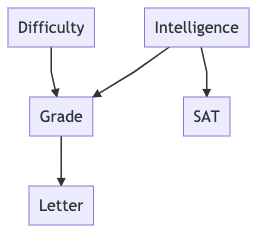
\includegraphics[width=\linewidth]{Figures/lic/student-network.png}
        \caption{Student scenario, \parencite{koller2009probabilistic}}
    \end{figure}
% graph TD
%   D[Difficulty] --> G[Grade]
%   I[Intelligence] --> G
%   I --> S[SAT]
%   G --> L[Letter]
\end{minipage}
\pause
\begin{minipage}{0.58\linewidth}
    \begin{verbatim}
    d ~ dPrior
    i ~ iPrior
    g ~ gCond(d, i)
    s ~ sCond(i)
    l ~ lCond(g)
    \end{verbatim}
\end{minipage}

\pause

\textbf{Example Query}: \texttt{infer(i, {l=Good, s=800})}

Given a student's recommendation \emph{letter} and \emph{SAT} score,
what should I expect their \emph{intelligence} to be?


\note[itemize]{
    \item Probabilistic model for student recommendation letters and SAT scores
    \item Priors and conditionals
    \item Observations (Letter, SAT), Queries (Intelligence)
}
\end{frame}

\begin{frame}[fragile]{Monte Carlo approximation}
\begin{align*}
    &\mathbb{E}[\text{Intelligence} | \text{Letter}=\text{Good}, \text{SAT}=1600] \\
    &= \int I \cdot \Pr[\text{Intelligence}=I | \text{Letter}=\text{Good}, \text{SAT}=1600] dI \\
    &\approx \frac{1}{N} \sum_{n=1}^N I_n
\end{align*}
where $I_n \sim \Pr[\text{Intelligence} | \text{Letter}=\text{Good}, \text{SAT}=1600]$

\note[itemize]{
\item Integrals are just really tiny sums, CLT $1/\sqrt{N}$ rate
\item Can answer this question by drawing samples from the posterior, inference is solved by sampling the posterior
}
\end{frame}

\begin{frame}[fragile]{Monte Carlo Markov Chain}
    How to sample? Consider producing $\{I_n\}$ by:
    \begin{itemize}
        \item Fix $\text{Letter}=\text{Good}$ and $\text{SAT}=1600$
        \item Repeat:
        \begin{itemize}
            \item UAR choose a latent variable to resample
            \item Sample a \emph{proposal distribution} $Q(\cdot)$ to propose a new value
            \item Accept with probability $\alpha$ and revert otherwise, emit $I_n$
        \end{itemize}
    \end{itemize}
    \pause
    \begin{theorem}[\cite{hastings1970monte}]
        With appropriately chosen $\alpha$, the above algorithm yields
        a Markov Chain with the posterior as the invariant distribution.
    \end{theorem}
\end{frame}

\subsection{Inference Compilation}

\begin{frame}[fragile]{Proposal distributions}
    Different $Q(\cdot)$ $\implies$ different MCMC algorithms
    
    \begin{itemize}
        \item Random walk MH: $Q(\cdot)$ isotropic Gaussian
        \item Newtonian Monte Carlo \parencite{arora2020newtonian}:
        $Q(\cdot) =$ Hessian-based Gaussian
        \item Hamiltonian Monte Carlo: $Q(\cdot)$ integrates dynamical system
        \item \emph{Inference Compilation}: $Q(\cdot)$ output of a neural network
    \end{itemize}
\end{frame}

\begin{frame}{Intuition for IC}
    \begin{figure}
        \centering
        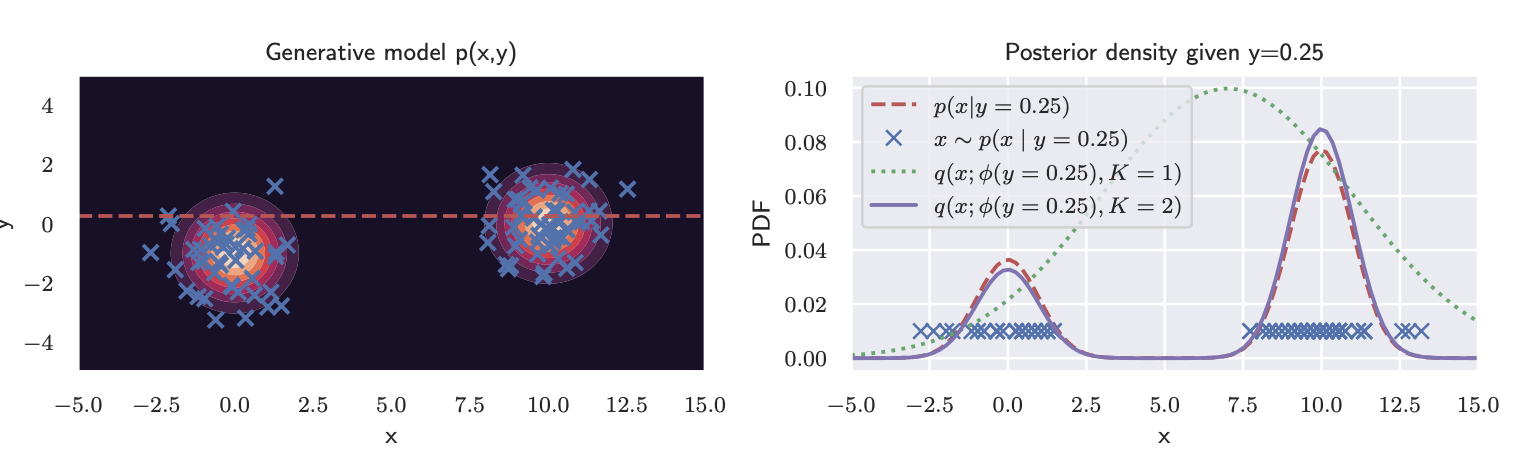
\includegraphics[width=\textwidth]{Figures/lic/intuition.png}
    \end{figure}
\end{frame}

\begin{frame}{Results: GMM mode escape}
    \begin{figure}
        \centering
        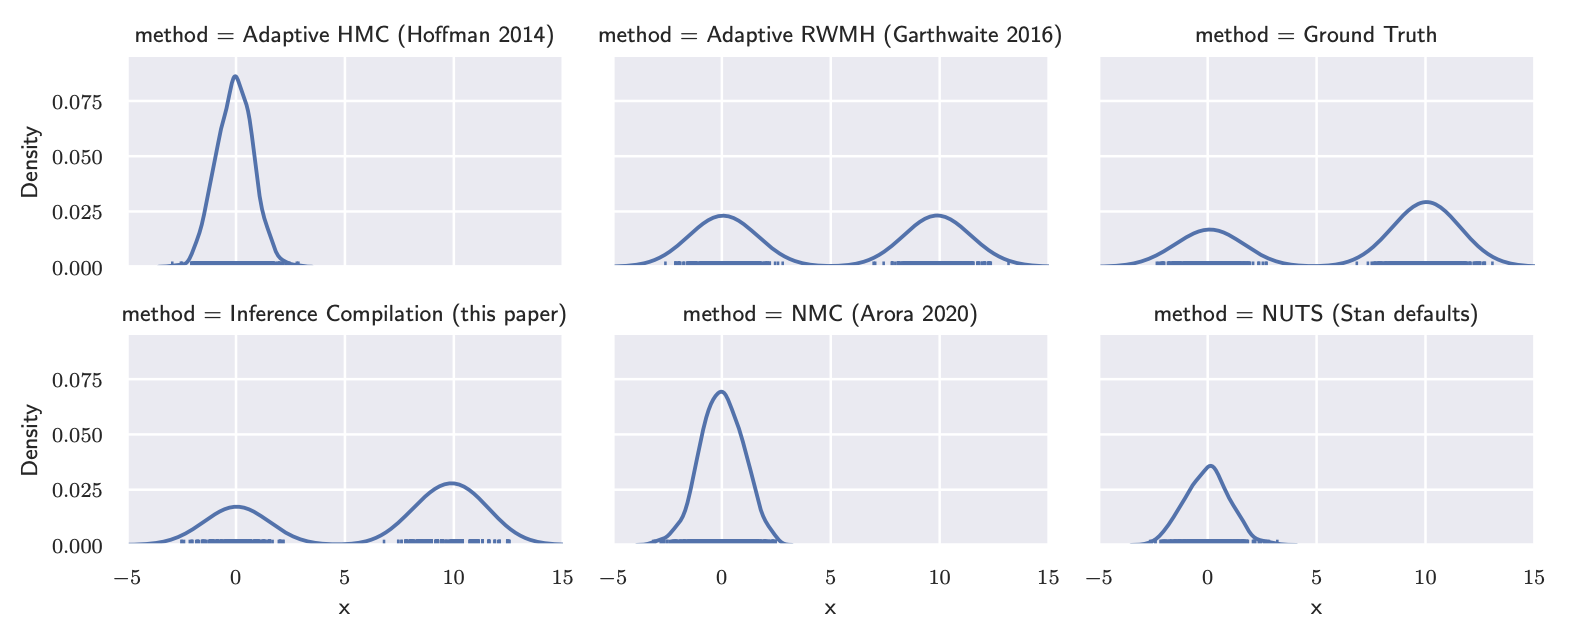
\includegraphics[width=\textwidth]{Figures/lic/gmm-escape.png}
    \end{figure}
\end{frame}

% \begin{frame}[fragile]{Prior work: IC in imperative PPLs}
% 	\begin{figure}
% 	    \centering
% 	    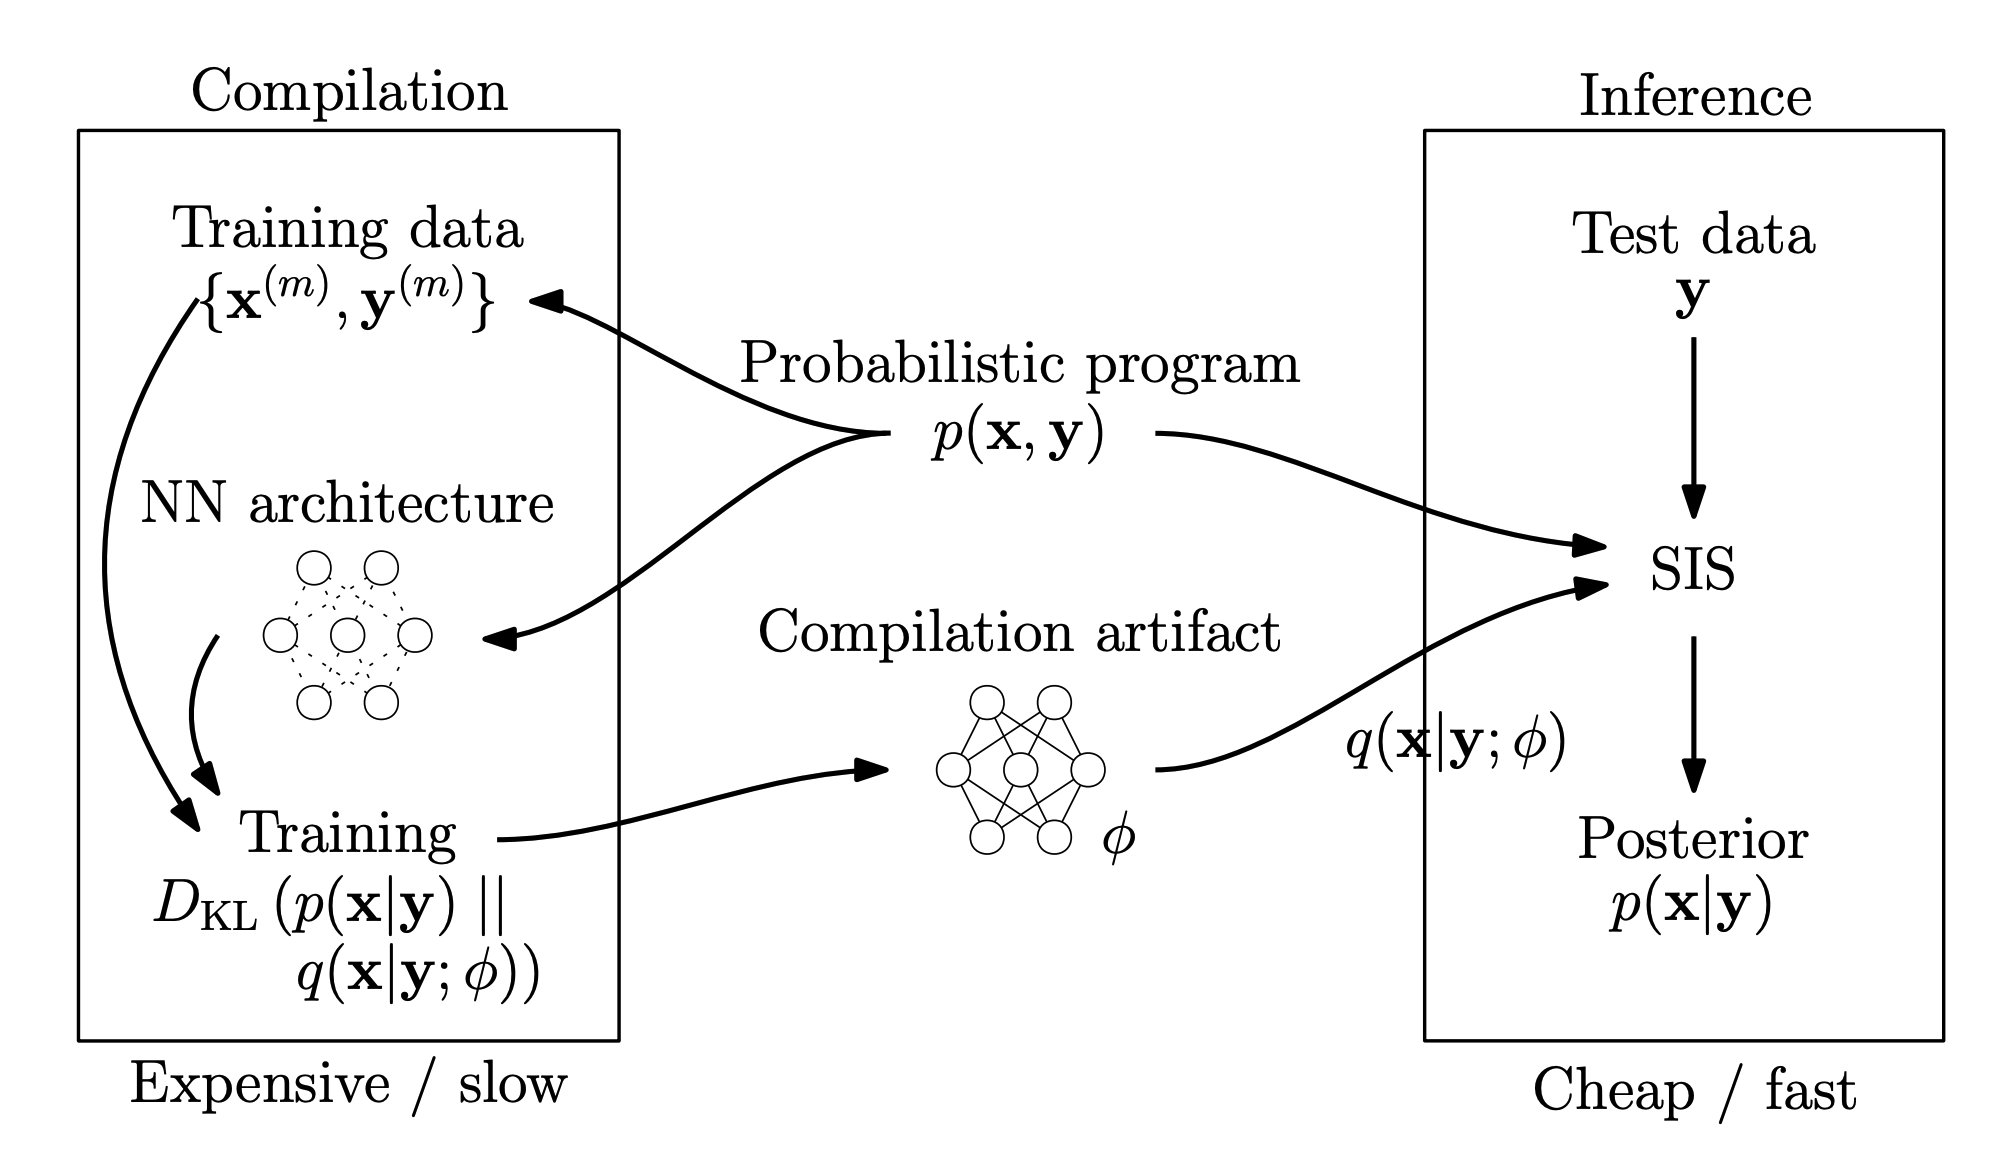
\includegraphics[width=0.7\linewidth]{Figures/lic/ic.png}
% 	    \caption{Inference compilation in SMC \cite{le2017inference}}
% 	\end{figure}
	
% 	\note[itemize]{
% 	\item Similar
% 	\begin{itemize}
% 	    \item Forward sampling of PP to generate training data
% 	    \item Minimize inclusive KL MC estimate from generated data
% 	    \item Amortize IC artifacts across many observations $\vec{y}$
% 	\end{itemize}
% 	\item Differences
% 	\begin{itemize}
% 	    \item SIS vs MH, minimal I-map
% 	\end{itemize}
% 	}
% \end{frame}

\begin{frame}[fragile]{Prior Work: RNN on execution trace \parencite{le2017inference}}
\begin{minipage}{0.4\linewidth}
    \begin{figure}
        \centering
        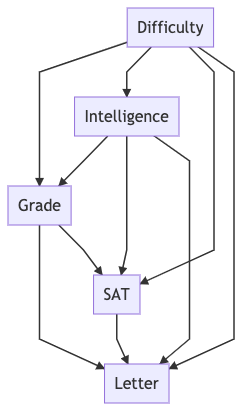
\includegraphics[width=\linewidth]{Figures/lic/student-network-smc-ic.png}
    \end{figure}
% graph TD
%   D[Difficulty] --> G[Grade]
%   D --> I
%   D --> S
%   D --> L
%   I[Intelligence] --> G
%   I --> S[SAT]
%   I --> L
%   G --> L[Letter]
%   G --> S
%   S --> L
\end{minipage}
\begin{minipage}{0.5\linewidth}
    \begin{align*}
        & q(d | \text{observations}) \\
        & q(i|d, \text{observations}) \\
        & q(g | i, d, \text{observations}) \\
        & q(s | g, i, d, \text{observations}) \\
        & q(l | s, g, i, d, \text{observations})
    \end{align*}
\end{minipage}
\end{frame}

\begin{frame}[fragile]{Our contribution: IC with minimal I-maps\footnote{\fullcite{liang2021accelerating}}}
    \begin{minipage}{0.4\linewidth}
    \begin{figure}
        \centering
        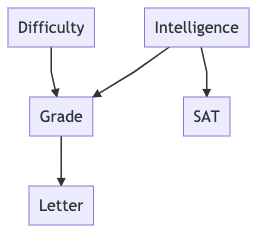
\includegraphics[width=\linewidth]{Figures/lic/student-network.png}
    \end{figure}
\end{minipage}
\begin{minipage}{0.5\linewidth}
\begin{align*}
    & q(d | g, i, \text{observations}) \\
    & q(i | g, d, s, \text{observations}) \\
    & q(g | i, d, l, \text{observations}) \\
    & q(s | i, \text{observations}) \\
    & q(l | g, \text{observations})
\end{align*}
\end{minipage}

``Deep sets'' \parencite{zaheer2017deep} applied to Markov Blanket


    \note[itemize]{
    \item Each IC proposer only has access to Markov Blanket, respects causal structure
    \item SIS IC suffers in presence of nuisance parameters, requires attention to perform well
    \item Explain declarative vs imperative (parents are clearly demarcated)
    }
\end{frame}


\begin{subframe}{Architecture}
    \begin{figure}
        \centering
        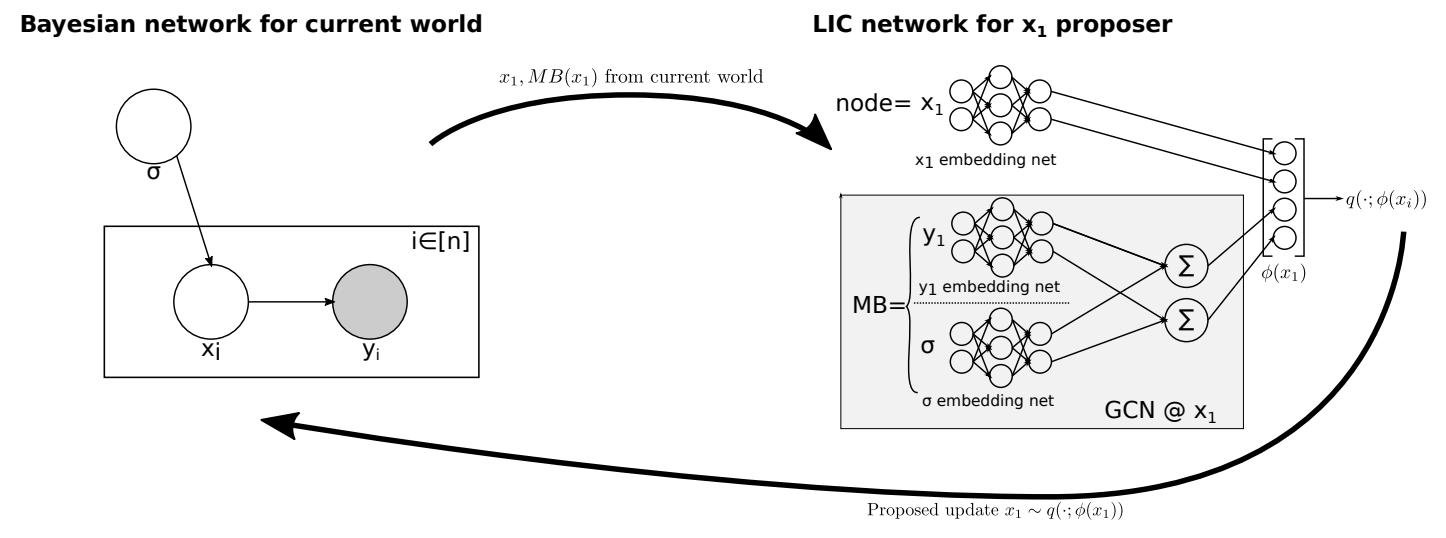
\includegraphics[width=\textwidth]{Figures/lic/schematic-eg.png}
    \end{figure}
    
    ``Deep sets'' \parencite{zaheer2017deep} applied to Markov Blanket
\end{subframe}


\begin{subframe}[fragile]{Example IC proposer for "grade"}

\begin{figure}
    \centering
    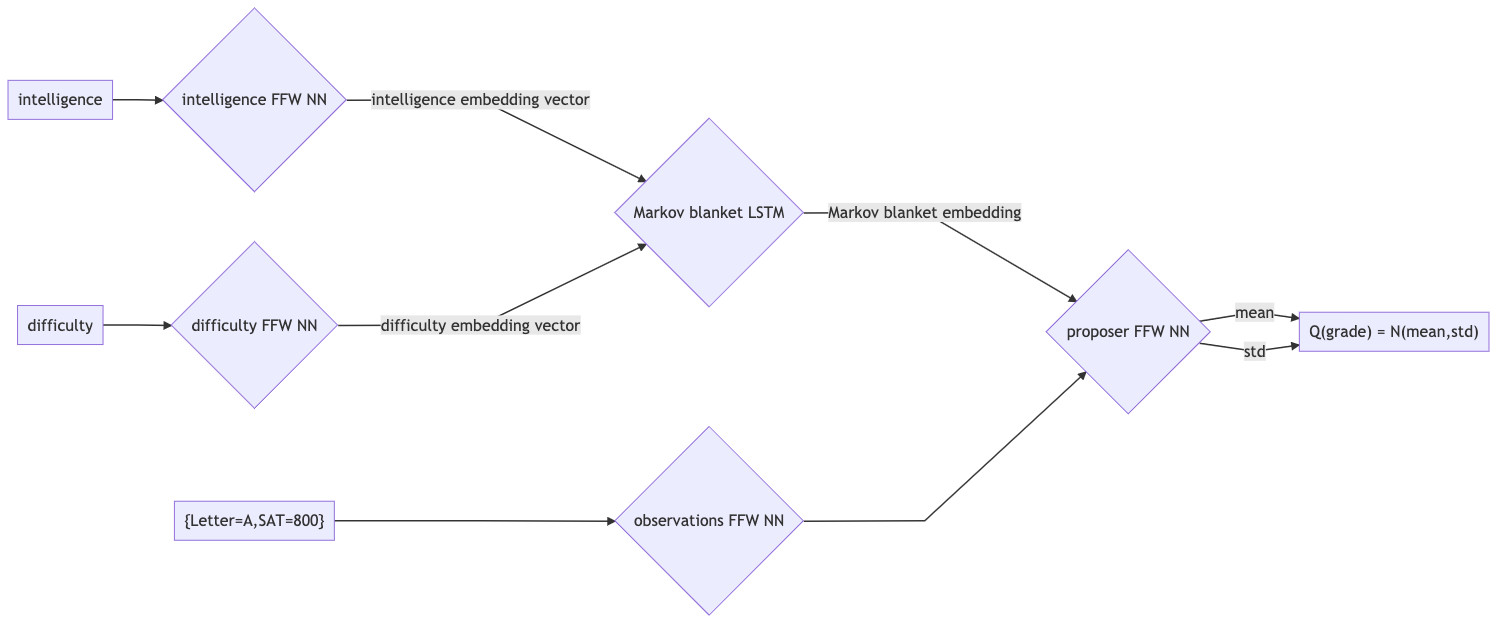
\includegraphics[width=\linewidth]{Figures/lic/ic-grade.png}
    \caption{IC proposer for \texttt{grade}}
% graph LR
% 	O["{Letter=A,SAT=800}"] --> Oe{observations FFW NN}
%   I[intelligence] --> Ie{intelligence FFW NN}
%   D[difficulty] --> De{difficulty FFW NN}
% 	Ie -->|intelligence  embedding vector| MB{Markov blanket LSTM}
%   De -->|difficulty embedding vector| MB
%   MB -->|Markov blanket embedding| P{proposer FFW NN}
%   Oe --> P
%   P -->|mean| Q["Q(grade) = N(mean,std)"]
%   P -->|std| Q
\end{figure}

\note[itemize]{
    \item Markov blanket can change size due to switching variables => LSTM
    \item Problem: density estimator currently Gaussian/Categorical
    \item Problem: observations shape fixed at compile
}
\end{subframe}




\begin{frame}{Results: nuisance parameter robustness}
    \begin{figure}[p]
        \centering
        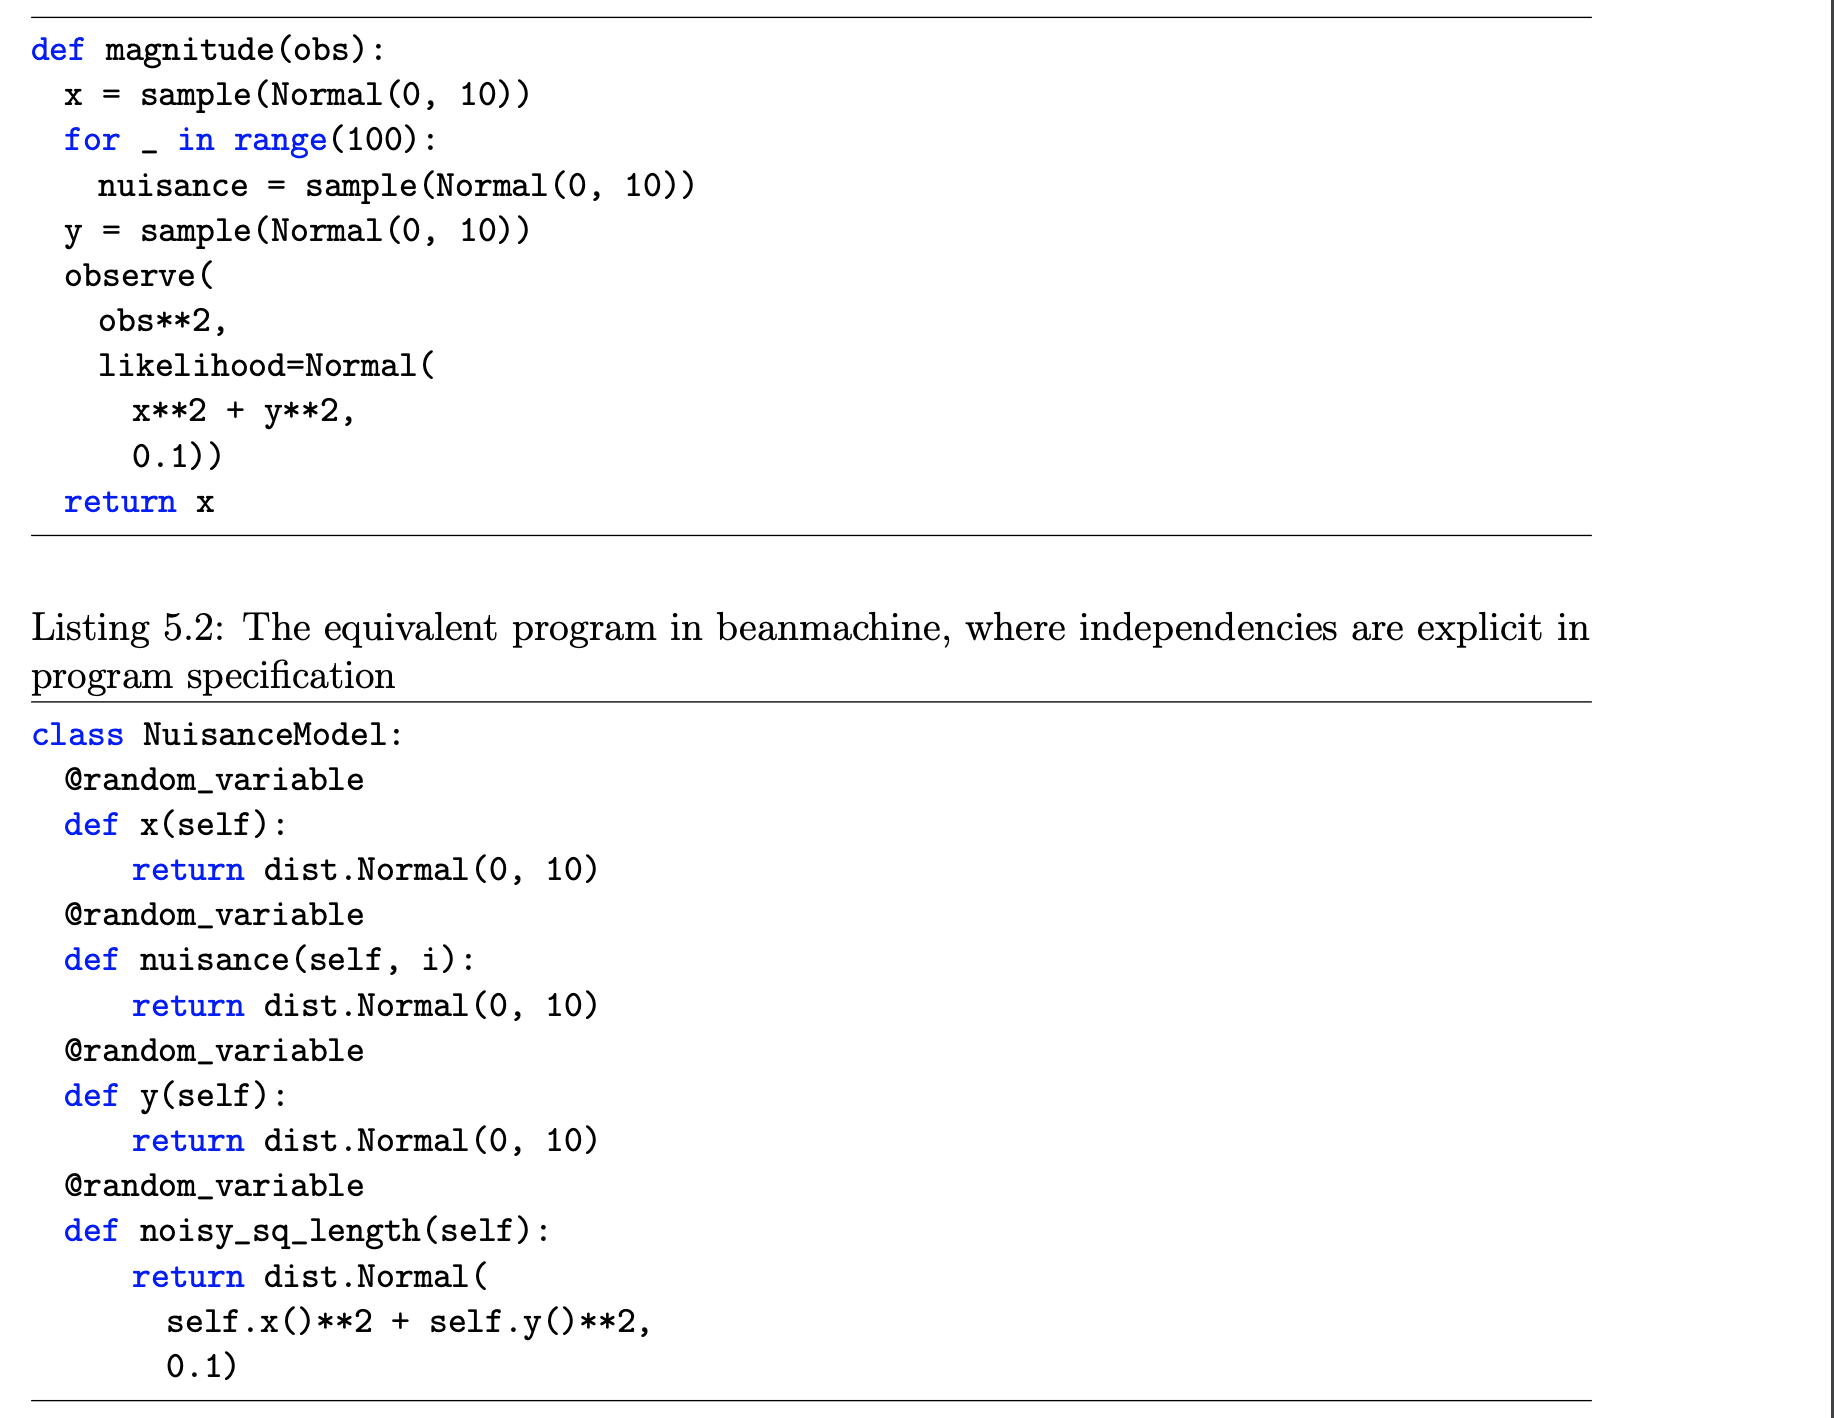
\includegraphics[width=0.4\textwidth,trim={0 16cm 20cm 0.5cm},clip]{Figures/lic/nuisance-progs.png}
        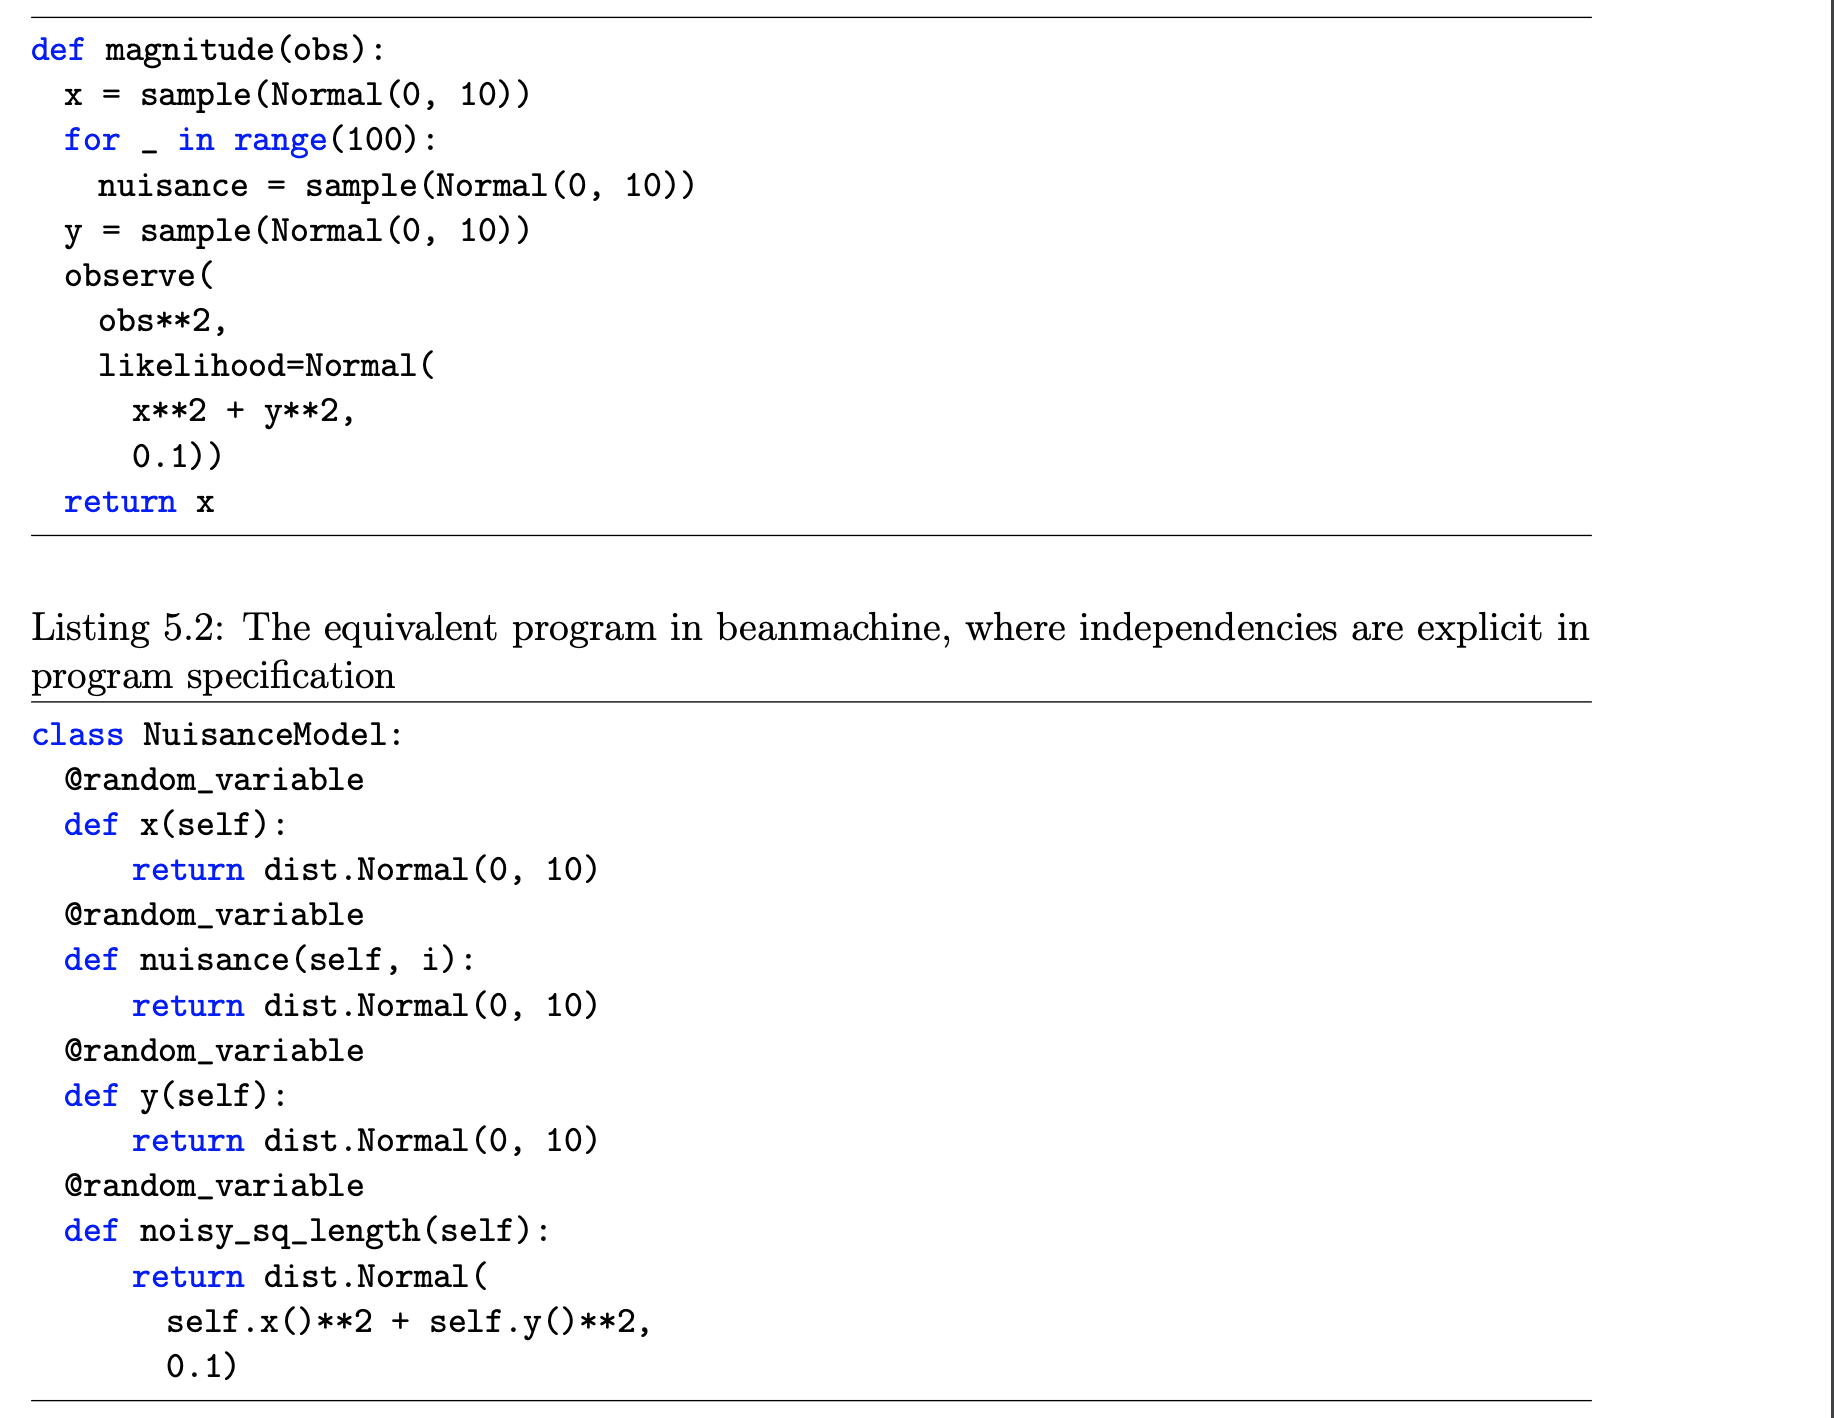
\includegraphics[width=0.4\textwidth,trim={0 0.5cm 20cm 12.5cm},clip]{Figures/lic/nuisance-progs.png}
    \end{figure}
    \begin{figure}
        \centering
        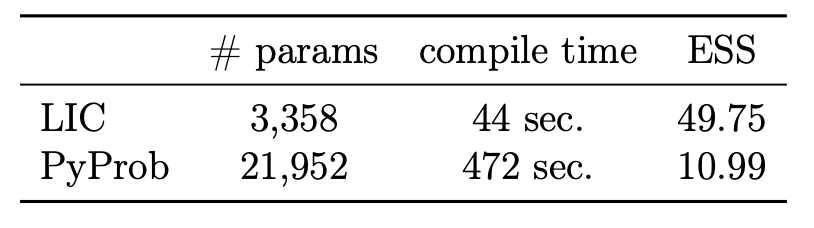
\includegraphics[width=0.6\textwidth]{Figures/lic/nuisance-params.png}
    \end{figure}
\end{frame}

\begin{frame}{Results: n-schools}
    \begin{figure}
        \centering
        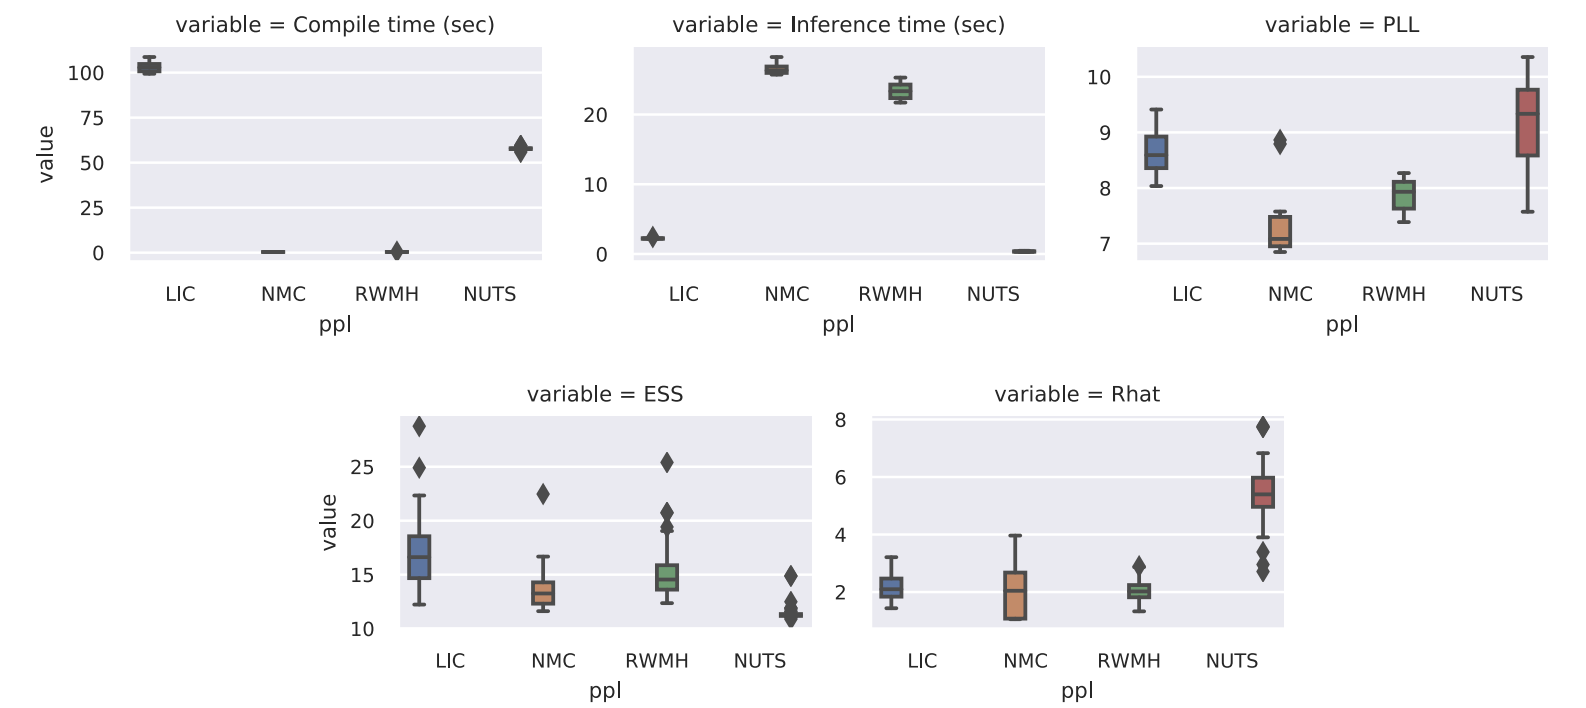
\includegraphics[width=\textwidth]{Figures/lic/nschools.png}
    \end{figure}
\end{frame}

\begin{subframe}{Results: Bayesian logistic regression}
    \begin{figure}
        \centering
        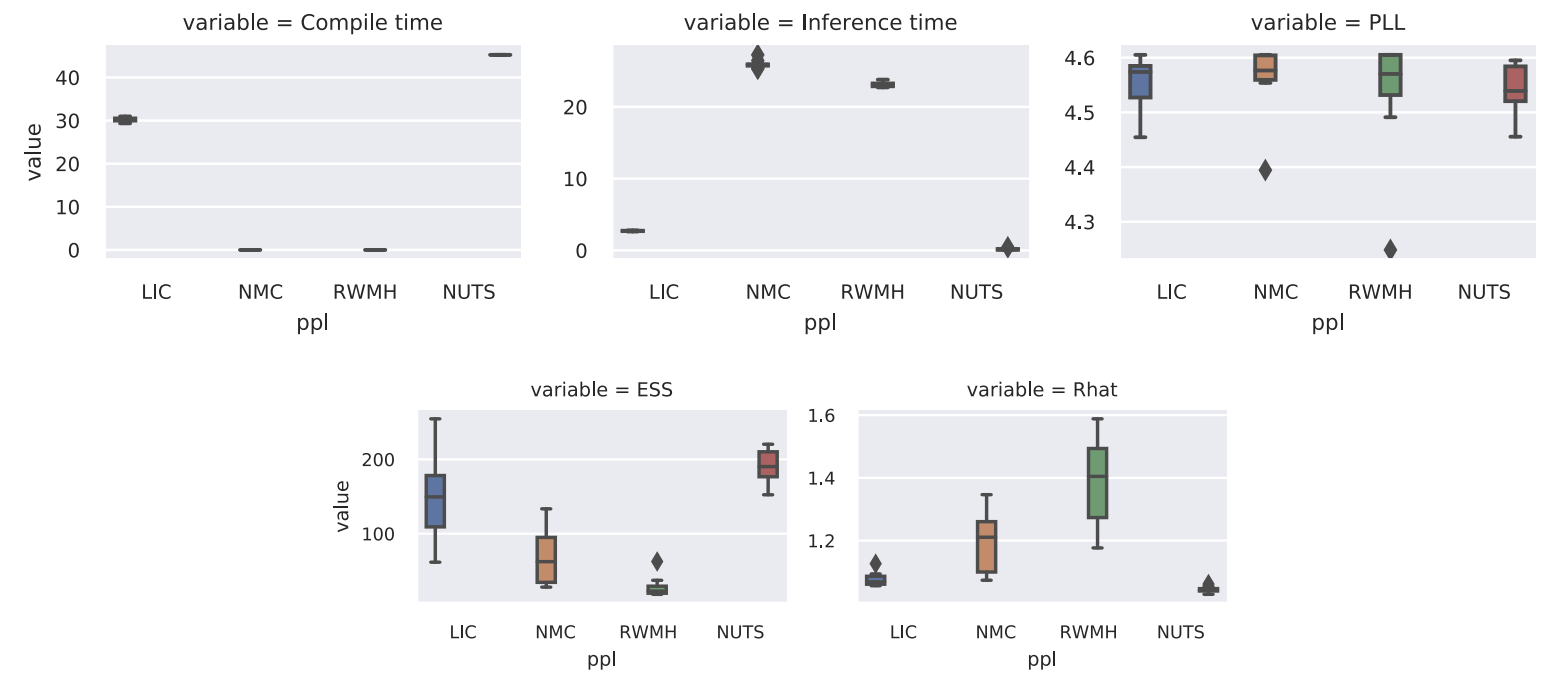
\includegraphics[width=\textwidth]{Figures/lic/blr.png}
    \end{figure}
\end{subframe}

% \begin{frame}[fragile]{Normal-normal model}
% 	$p \sim N(0.0, 2.0)$, $x \sim N(p, 0.1)$,
	
% 	\textbf{Goal}: Draw samples $\Pr[p \mid x]$
	
% 	\textbf{Conjugacy}: Calculus shows $\Pr[p \mid x] = N(0.9975 x, 0.009975)$,
% 	member of variational family $\implies$ zero approximation error
	
% 	\note[itemize]{
% 	    \item Conjugate model where we know exact result is a precision weighted average
% 	    \item Posterior is normal, in variational family, no approximation error
% 	}
% \end{frame}

% \begin{frame}[fragile]{Random walk MH on Normal-Normal model}
%     \begin{figure}
%         \centering
%         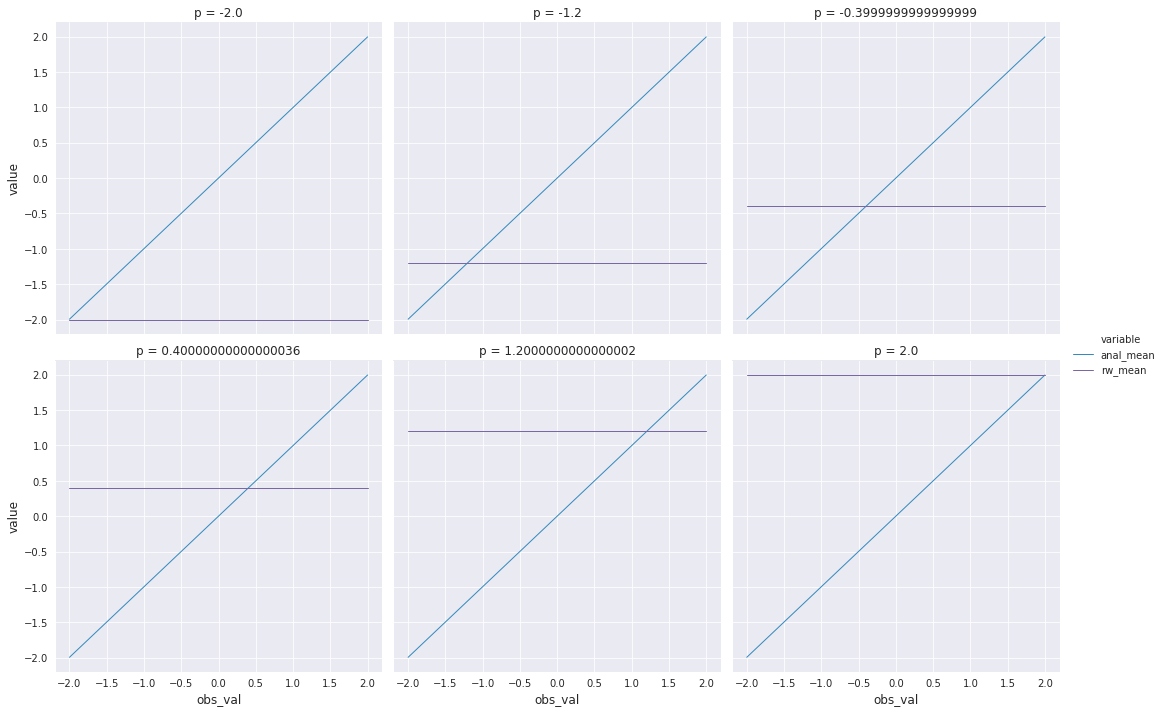
\includegraphics[width=\linewidth]{Figures/lic/rwmh.png}
%         \caption{Random walk MH's proposer mean depends on current value of $p$ in Markov chain}
%     \end{figure}
% \end{frame}

% \begin{frame}[fragile]{IC on Normal-Normal model: the good parts}
%     \begin{figure}
%         \centering
%         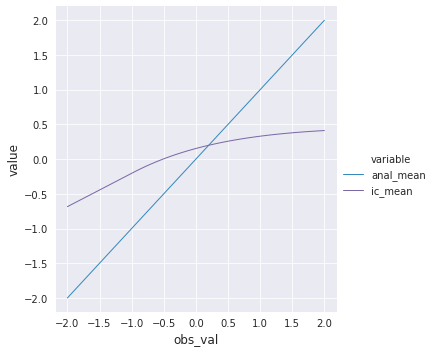
\includegraphics[width=0.7\linewidth]{Figures/lic/ic_normal_normal.png}
%         \caption{IC on Normal-Normal successfully captures posterior mean [n313855]}
%     \end{figure}
%     \note[itemize]{
%     \item Does not depend on current value of $p$
%     }
% \end{frame}

% \begin{frame}[fragile]{IC on Normal-Normal model: the bad parts}
%     Sensitive to initialization
%     \begin{figure}
%         \centering
%         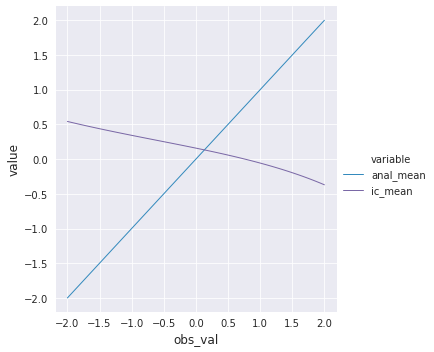
\includegraphics[width=0.48\linewidth]{Figures/lic/ic_normal_normal_fail_mean.png}
%         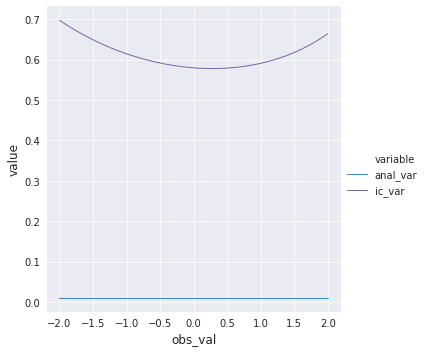
\includegraphics[width=0.48\linewidth]{Figures/lic/ic_normal_normal_fail_var.png}
%         \caption{Exploding variance on bad initializations [n313855]}
%     \end{figure}
%     \note[itemize]{
%         \item Depends on initialization, sometimes optimization explodes variance to maximize probability
%         \item NOTE: bad variational approximation could still give decent MCMC results; proposer covers support of posterior
%     }
% \end{frame}

% \begin{frame}[fragile]{IC on Normal-Normal model: the bad parts}
%     Local optima problems mitigated by reducing model parameters
%     \begin{figure}
%         \centering
%         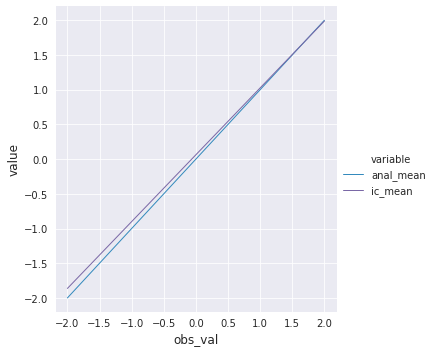
\includegraphics[width=0.6\linewidth]{Figures/lic/ic_normal_normal_linear.png}
%         \caption{IC with appropriate model size accurately captures posterior mean [n313855]}
%     \end{figure}
%     \note[itemize]{
%         \item 1D observation embedding, no activation functions => can only learn linear functions
%         \item Works here, but not general. Will look at regularization to reduce hypothesis space later.
%     }
% \end{frame}


% \begin{frame}[fragile]{Vectorized n-schools}
% 	\begin{figure}
% 	    \centering
% 	    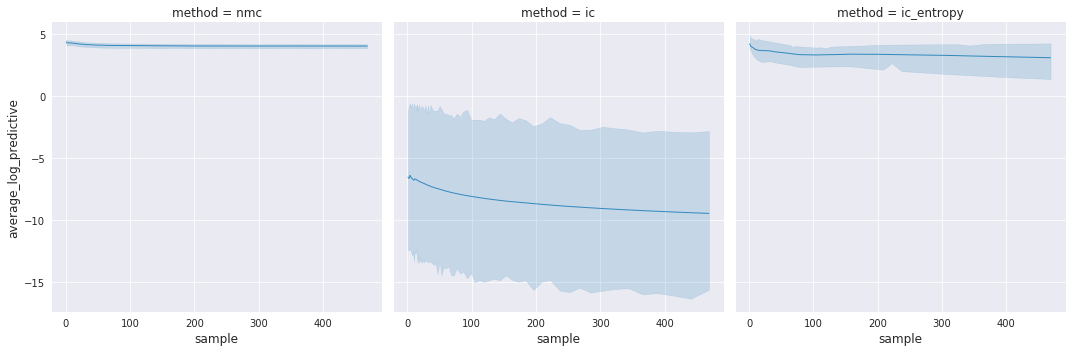
\includegraphics[width=0.9\linewidth]{Figures/lic/nschools-pll.png}
% 	    \caption{Predictive log likelihoods on vectorized n-schools [D22448718]}
% 	\end{figure}
% \end{frame}

% \begin{frame}[fragile]{Vectorized n-schools}
% 	\begin{figure}
% 	    \centering
% 	    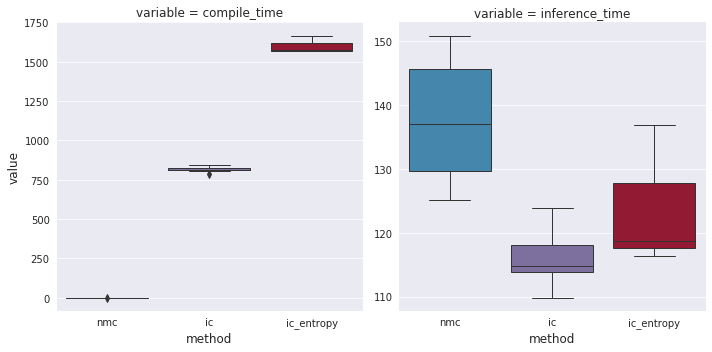
\includegraphics[width=0.7\linewidth]{Figures/lic/nschools-compile-infer-time.png}
% 	    \caption{IC amortizes compilation costs (10,000 worlds above) through faster inference runtimes}
% 	\end{figure}
% \end{frame}

% \begin{frame}[fragile]{Vectorized n-schools}
% 	\begin{figure}
% 	    \centering
% 	    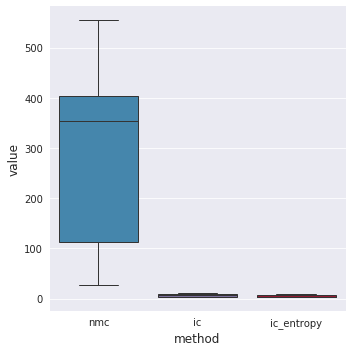
\includegraphics[width=0.4\linewidth]{Figures/lic/nschools-ic-neff.png}
% 	    \caption{IC yields very low ESS (no burn in, 500 samples)}
% 	\end{figure}
% \end{frame}

% \subsection{Limitations and next steps}

% \begin{frame}[fragile]{Limitations and next steps}
%     \begin{itemize}
%         \item Other variational families (eg GMM, IAF)
%         \item Entropy regularization to address exploding variance
%         \begin{align*}
%             \mathcal{L}(\phi)
%             &= D_{KL}(p(\vec{x} \mid \vec{y}) || q(\vec{x} \mid \vec{y}; \phi) ) + H(q(\vec{x} \mid \vec{y}; \phi))
%         \end{align*}
%     \end{itemize}
    
%     \begin{figure}
%         \centering
%         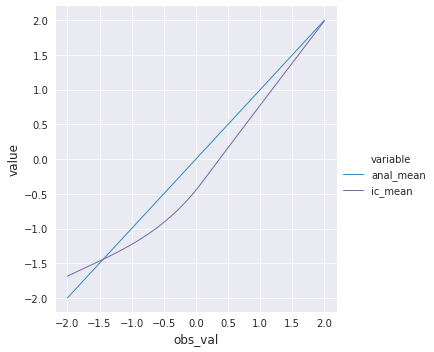
\includegraphics[width=0.4\linewidth]{Figures/lic/ic-entropy-mean.png}
%         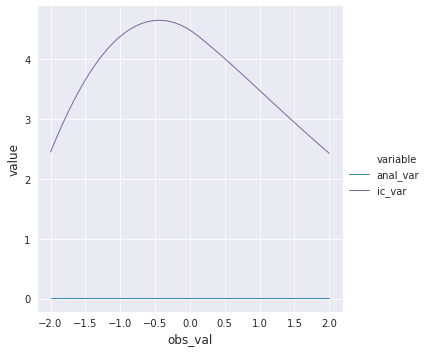
\includegraphics[width=0.4\linewidth]{Figures/lic/ic-entropy-var.png}
%         \caption{Entropy regularization penalizes exploding variance, favoring a better variational approximation in Normal-Normal
%         [n313855]}
%     \end{figure}

% 	\note[itemize]{
% 	    \item Currently only diagonal normal (mean-field) and categorical variational families, GMM and IAF can both capture multimodal densities as well as correlations
% 	    \item Entropy regularization penalizes exploding variance; how to theoretically justify?
% 	}
% \end{frame}


% \appendix


% \begin{frame}[fragile]{Contribution: Online Adaptation}
%     \textbf{Problem}: forward samples during compilation may not sufficiently represent observations ($\text{obs}$) encountered at inference
    
%     \textbf{Solution}: perform MCMC with IC artifact to draw posterior samples $(\vec{x}^{(m)}, \vec{y}^{(m)}=\text{obs}) \sim P(\vec{x} \mid \vec{y}=\text{obs})$,
%     hill-climb inclusive KL between \emph{conditional} (rather than joint) posterior
%     \begin{align*}
%         &\argmin_{\phi} D_{KL}(p(\vec{x} | \vec{y}=\text{obs}) || q(\vec{x} | \vec{y}=\text{obs}; \phi)) \\
%         &\approx 
%         \argmin_{\phi} \sum_{m=1}^N \log Q(\vec{x}^{(m)} \mid \vec{y} = \text{obs}, \phi)
%     \end{align*}
% \end{frame}


% \begin{frame}[fragile]{IC on Normal-Normal model: the bad parts}
%     Also affects \cite{le2017inference}
%     \begin{figure}
%         \centering
%         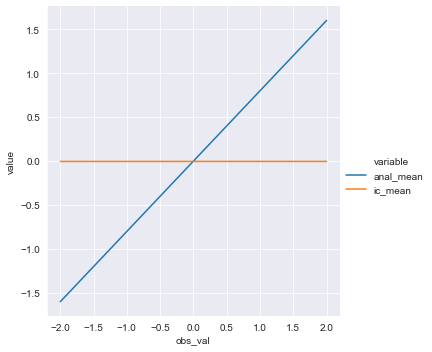
\includegraphics[width=0.48\textwidth]{Figures/lic/ic-smc-fail.png}
%         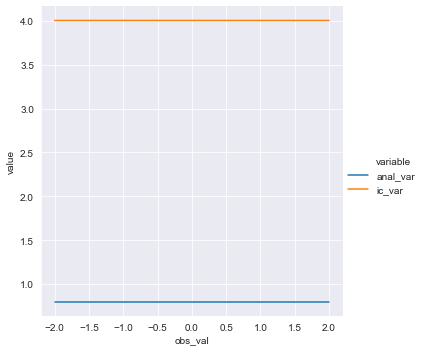
\includegraphics[width=0.48\textwidth]{Figures/lic/ic-smc-fail-var.png}
%         \caption{\texttt{pyprob}'s\footnote{\tiny\url{https://github.com/pyprob/pyprob/}} IC also exhibits variance explosion
%         \footnote{\tiny\url{https://github.com/facebookexternal/ppl_papers/blob/master/ic/Normal-Normal\%20convergence\%20studies.ipynb
%         }}}
%     \end{figure}
% \end{frame}